%%%%%%%%%%%%%%%%%%%%%%%%%%%%%%%%%%%%%%%%%
% a0poster Portrait Poster
% LaTeX Template
% Version 1.0 (22/06/13)
%
% The a0poster class was created by:
% Gerlinde Kettl and Matthias Weiser (tex@kettl.de)
% 
% This template has been downloaded from:
% http://www.LaTeXTemplates.com
%
% License:
% CC BY-NC-SA 3.0 (http://creativecommons.org/licenses/by-nc-sa/3.0/)
%
%%%%%%%%%%%%%%%%%%%%%%%%%%%%%%%%%%%%%%%%%

%----------------------------------------------------------------------------------------
%	PACKAGES AND OTHER DOCUMENT CONFIGURATIONS
%----------------------------------------------------------------------------------------

\documentclass[a0, portrait]{a0poster}

\usepackage{multicol} % This is so we can have multiple columns of text side-by-side
\columnsep=100pt % This is the amount of white space between the columns in the poster
\columnseprule=3pt % This is the thickness of the black line between the columns in the poster

\usepackage[svgnames]{xcolor} % Specify colors by their 'svgnames', for a full list of all colors available see here: http://www.latextemplates.com/svgnames-colors

\usepackage{times} % Use the times font
%\usepackage{palatino} % Uncomment to use the Palatino font

\usepackage{graphicx} % Required for including images
\graphicspath{{figures/}} % Location of the graphics files
\usepackage{booktabs} % Top and bottom rules for table
\usepackage[font=small,labelfont=bf]{caption} % Required for specifying captions to tables and figures
\usepackage{amsfonts, amsmath, amsthm, amssymb} % For math fonts, symbols and environments
\usepackage{wrapfig} % Allows wrapping text around tables and figures

\usepackage{balance} % for balancing columns on the final page
\usepackage{xspace}
\usepackage{caption}
\usepackage{subcaption}
\usepackage[fontsize=27.6pt]{fontsize}



% Shaded blocks.
\usepackage{framed,xcolor}
\colorlet{shadecolor}{orange!15}

\newcommand{\BibTeX}{\rm B\kern-.05em{\sc i\kern-.025em b}\kern-.08em\TeX}

\newcommand{\SA}{\emph{SA}\xspace}
\newcommand{\SAM}{\emph{$SA_M$}\xspace}

\begin{document}

%----------------------------------------------------------------------------------------
%	POSTER HEADER 
%----------------------------------------------------------------------------------------

% The header is divided into two boxes:
% The first is 75% wide and houses the title, subtitle, names, university/organization and contact information
% The second is 25% wide and houses a logo for your university/organization or a photo of you
% The widths of these boxes can be easily edited to accommodate your content as you see fit

\begin{minipage}[b]{0.75\linewidth}
\veryHuge \color{NavyBlue} \textbf{Intention Progression with Maintenance Goals} \color{Black}\\ % Title
% \Huge\textit{An Exploration of Complexity}\\[2cm] % Subtitle
\huge \textbf{Di Wu \& Yuan Yao \& Natasha Alechina \& Brian Logan \& John Thangarajah}\\[0.5cm] % Author(s)
\huge Zhejiang University of Techonology \& University of Nottingham Ningbo\\[0.4cm] % University/organization
% \Large \texttt{wudi@zjut.edu.cn} \&
% \Large \texttt{yuan.yao@nottingham.edu.cn}
\end{minipage}
%
\begin{minipage}[b]{0.25\linewidth}
% 
\includegraphics[width=20cm]{logo.png}\\
\end{minipage}

\vspace{1cm} % A bit of extra whitespace between the header and poster content

%----------------------------------------------------------------------------------------

\begin{multicols}{3} % This is how many columns your poster will be broken into, a portrait poster is generally split into 2 columns

%----------------------------------------------------------------------------------------
%	ABSTRACT
%----------------------------------------------------------------------------------------

% \color{Navy} % Navy color for the abstract

%----------------------------------------------------------------------------------------
%	INTRODUCTION
%----------------------------------------------------------------------------------------

% \color{SaddleBrown} % SaddleBrown color for the introduction

In this paper, we propose \SAM, a Monte-Carlo Tree Search (MCTS)-based solver for intention progression problem with both achievement and maintenance goals. We evaluate the performance of our approach in a range of benchmark scenarios with increasing difficulty. The results suggest that \SAM significantly improves the performance of agents with maintenance goals.


One of the key advantages of Belief-Desire-Intention (BDI) agents \cite{Rao/Georgeff:92a} is their ability to pursue multiple goals in parallel.
%
When multiple goals are pursued at the same time,  an agent has to decide which of its intentions should be progressed, and if the next step of the selected intention is a subgoal, the agent also has to decide which plan should be used. These two choices together form the \textit{intention progression problem} \cite{Logan//:17a}.
%
Existing works on intention progression problem are limited to scheduling achievement goals. In many applications agents must also \emph{maintain} particular states of the environment, e.g., not running out of power, avoiding collisions, etc., in addition to achieving certain states.
% definition
Such goals are termed \textit{maintenance goals}, as they specify a state of the environment an agent should maintain. 
%Maintenance goals have been already implemented in BDI systems such as Jadex \cite{Pokahr//:05a} and JAM\cite{Huber99}.
%\footnote{Maintenance goals have been already implemented in BDI systems such as Jadex \cite{Pokahr//:05a} and JAM\cite{Huber99}}
% Previous work.
Previous work \cite{DuffHT06} on proactively reasoning about maintenance goals is summary-information-based. However, that approach assumes that the preventive measure to maintain the goal doesn't interact with the agent's other intentions.

Here, we present \SAM, a new approach to intention progression for BDI agents with both achievement and maintenance goals.

% Contributions
% In this paper, we present \SAM, a new approach to intention progression for BDI agents with both achievement and maintenance goals, which extends \SA scheduler \cite{Yao//:16a}. 
%
% We compare the performance of our approach to that of \cite{DuffHT06}. The results suggest our approach significantly improves the performance of agents with maintenance goals.

%----------------------------------------------------------------------------------------
%	OBJECTIVES
%----------------------------------------------------------------------------------------

\color{DarkSlateGray} % DarkSlateGray color for the rest of the content

% \section*{Research Question}
% How to efficiently schedule BDI agent's intentions with both achievement and maintenance goals.


%----------------------------------------------------------------------------------------
%	MATERIALS AND METHODS
%----------------------------------------------------------------------------------------

\section*{Methods}

\SAM extends the \SA scheduler \cite{Yao/Logan:16a} in explicitly taking account of the agent's reactive and proactive maintenance goals.
%
\SAM is based on the Monte-Carlo Tree Search(MCTS) which uses pseudo-random simulations to guide the expansion of the search tree.
% edge
Edges in the search tree represent a choice of which action to execute in one of the agent's intentions.
% node
Each node is the state of the agent and its environment following the execution of the action.
% build search tree
% Starting from a root node representing the current state of the agent's intentions \emph{I} and state of the environment \emph{E}, \SAM iteratively builds a search tree until a pre-defined computational budget is reached, the scheduler then halts and the best action is returned. The intention \emph{I} is represented as a tuple $(T, S)$, where $T = \{t_1, ..., t_n\}$ is a set of goal-plan trees \cite{Thangarajah//:03a, Thangarajah//:11a, Yao//:16b} corresponding to the agent's top-level goals and $S=\{s_1, ..., s_n\}$ is a set of pointer to the current step of each goal-plan tree in $T$.
%
As with MCTS and \SA, each iteration of \SAM consists of four main phases: selection, expansion, simulation, and back-propagation.

To support intention progression with maintenance goals, we modified the expansion and the simulation phases of the \SA scheduler.
%In particular, the changes have been made to include a mechanism which decides when the recovery plans should be considered and how they should be executed.
%
\paragraph*{Modification to the expansion phase of \SA}
%
In the expansion phase of \SAM, different mechanisms are used for reactive and proactive maintenance goals.
%
For reactive maintenance goals, \SAM first checks if any of the maintenance conditions are violated in $n_s$ (the leaf node selected in the selection phase).
%
For each maintenance goal $G_m$ which has its maintenance condition violated in $n_s$,
a set of nodes representing the states resulting from executing each of its applicable recovery plans are generated, and added as the children of $n_s$.
%
% That is, in node $n_s$, the agent can choose either to continue achieving its top-level goals as before, or to execute recovery plans to re-establish the violated maintenance condition.
% The execution of recovery plans is not allowed, if the corresponding maintenance goals are not triggered.
%
For proactive maintenance goals, \SAM assumes maintenance goals are always active, i.e., it is always possible to execute a recovery plan for a maintenance goal $G_m$ if there is no existing intention for recovering $G_m$ yet.
%
In a special case when an agent does not have any achievement goals and all the maintenance conditions are not violated, no child node of $n_s$ will be generated. That is, if the agent is not pursuing any goals, then waiting is the best way to maintain the current state.
%
\paragraph{\textbf{Modifications to the Simulation Phase of \SA}}
During the simulation phase, \SAM randomly simulates the possible actions in achieving the agent's goals as in \SA. When the maintenance condition of a reactive maintenance goal $G_m$ is triggered, in addition to achieving the agent's achievement goals, \SAM can also select to execute the actions in one of $G_m$'s recovery plans.
%
For proactive maintenance goals, \SAM is able to execute their recovery plans anytime when there is no existing intention to maintain the same goals. The recovery plans for maintenance goals can also be interleaved with other intentions so as to avoid conflicts or to exploit synergies. %as in \cite{Yao/Logan:16a,Yao//:16a}.
%
The simulation ends when a terminal state is reached which contains one of the following situations:
1) All achievement goals are achieved and the maintenance condition is not violated.
2) All the remaining achievement goals cannot be achieved in the current state.
3) A maintenance condition cannot be re-established.


%----------------------------------------------------------------------------------------
%	RESULTS 
%----------------------------------------------------------------------------------------

\section*{Results}
We evaluate the performance of \SAM based on a Mars rover example \cite{DuffHT06}. The environment is a grid consisting of 20 $\times$ 20 cells (see Figure \ref{fig:marsrover}).

\begin{center}\vspace{1cm}
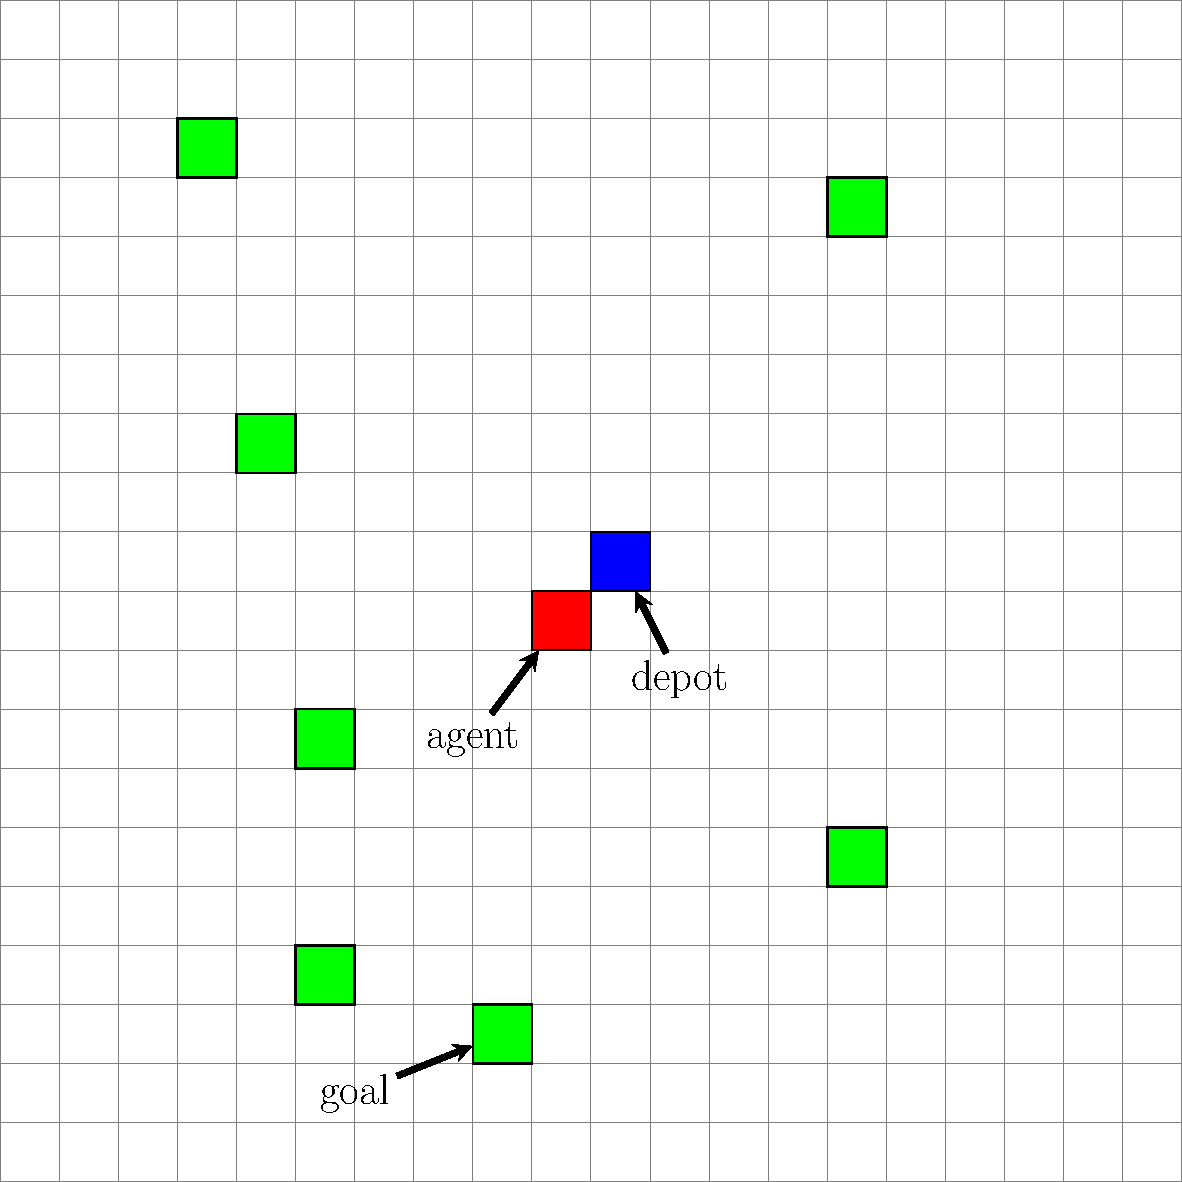
\includegraphics[scale=1]{./figs/mg_example.pdf}
\captionof{figure}{A Mars rover example}
\label{fig:marsrover}
\end{center}\vspace{1cm}
% introduction to the Mars rover example
%Each cell in the grid is a location represented as a pair of integer numbers (x, y), where x and y are the x-axis and y-axis values respectively.
%
%We assume the cell at the bottom-left corner is (0, 0) and the one at the top-right corner is (19, 19).
% 
%A Mars rover can move up, move down, move left and move right, and is asked to visit different locations in the grid.
%There are four actions the Mars rover agent can take to change its current locations, i.e., moveUp, moveDown, moveLeft and moveRight.%, which moves the Mars rover one cell up, down, left, and right respectively. 
% 
%In addition, each movement action will consume 1 unit of battery power. The Mars rover can move to the depot at the center to recharge its battery.
%

%In all the experiments reported below, we assume the Mars rover starts in the depot cell, and all its goals (i.e., where to visit) are randomly generated.
% measuring the agent
We measure the performance of the Mars rover agent based on two criteria: the number of goals achieved and the amount of battery consumed.
% That is, the performance of the agent will first be evaluated based on the number of achievement goals achieved (the more the better), if the same number of goals are achieved by different agents, we then compare their battery consumption for achieving the goals (the less the better).
To evaluate the performance of \SAM, the experiments were conducted in 4 cases: RMG, PMG, RMCTS and PMCTS.
%
Both RMG and PMG are from \cite{DuffHT06}.
%
%NMG means no maintenance goals: it assumes movement does not consume battery power. The agent achieves its goals in a FIFO manner.
%
%In the case of RMG, maintenance goals are handled reactively. When this reactive maintenance goal is triggered, the rover must first head to the depot to recharge its battery before attempting to achieve other goals.
%
%On the other hand, maintenance goals are handled proactively in PMG. The maintenance condition is predicted by using summary information. 
%
%NMCTS, as NMG, assumes no maintenance goals, but the goals are scheduled using the \SA scheduler.
%
%Both RMCTS and PMCTS use \SAM to schedule the progression of the agent's intentions. In RMCTS the maintenance goals are implemented reactively and in PMCTS proactively. 


%In the experiments, the \SAM and \SA schedulers are configured to perform 100 iterations in each deliberation cycle and 10 simulations per iteration; we report the average performance in 100 runs. The utility function is set to be $\#goals + \frac{1}{1 + \text{\emph{battery}}}$, where $\#goals$ is the number of goals achieved and \emph{battery} represents the amount of battery used to achieve the goals. We use the amount of battery consumption as additional measure of performance since all the approaches can achieve all goals. We set the battery capacity of the agent to 40 and vary the number of goals to be achieved from 1 to 15.
%
%The reactive maintenance condition is set to be \emph{batteryLevel} $> 20$. 
 %
%For proactive maintenance goals, the condition is set to be \emph{batteryLevel} greater than the minimal number of moves required for the agent to move back to the depot from its current position.

The results are shown in Figure \ref{fig:static1}.

\begin{center}\vspace{1cm}
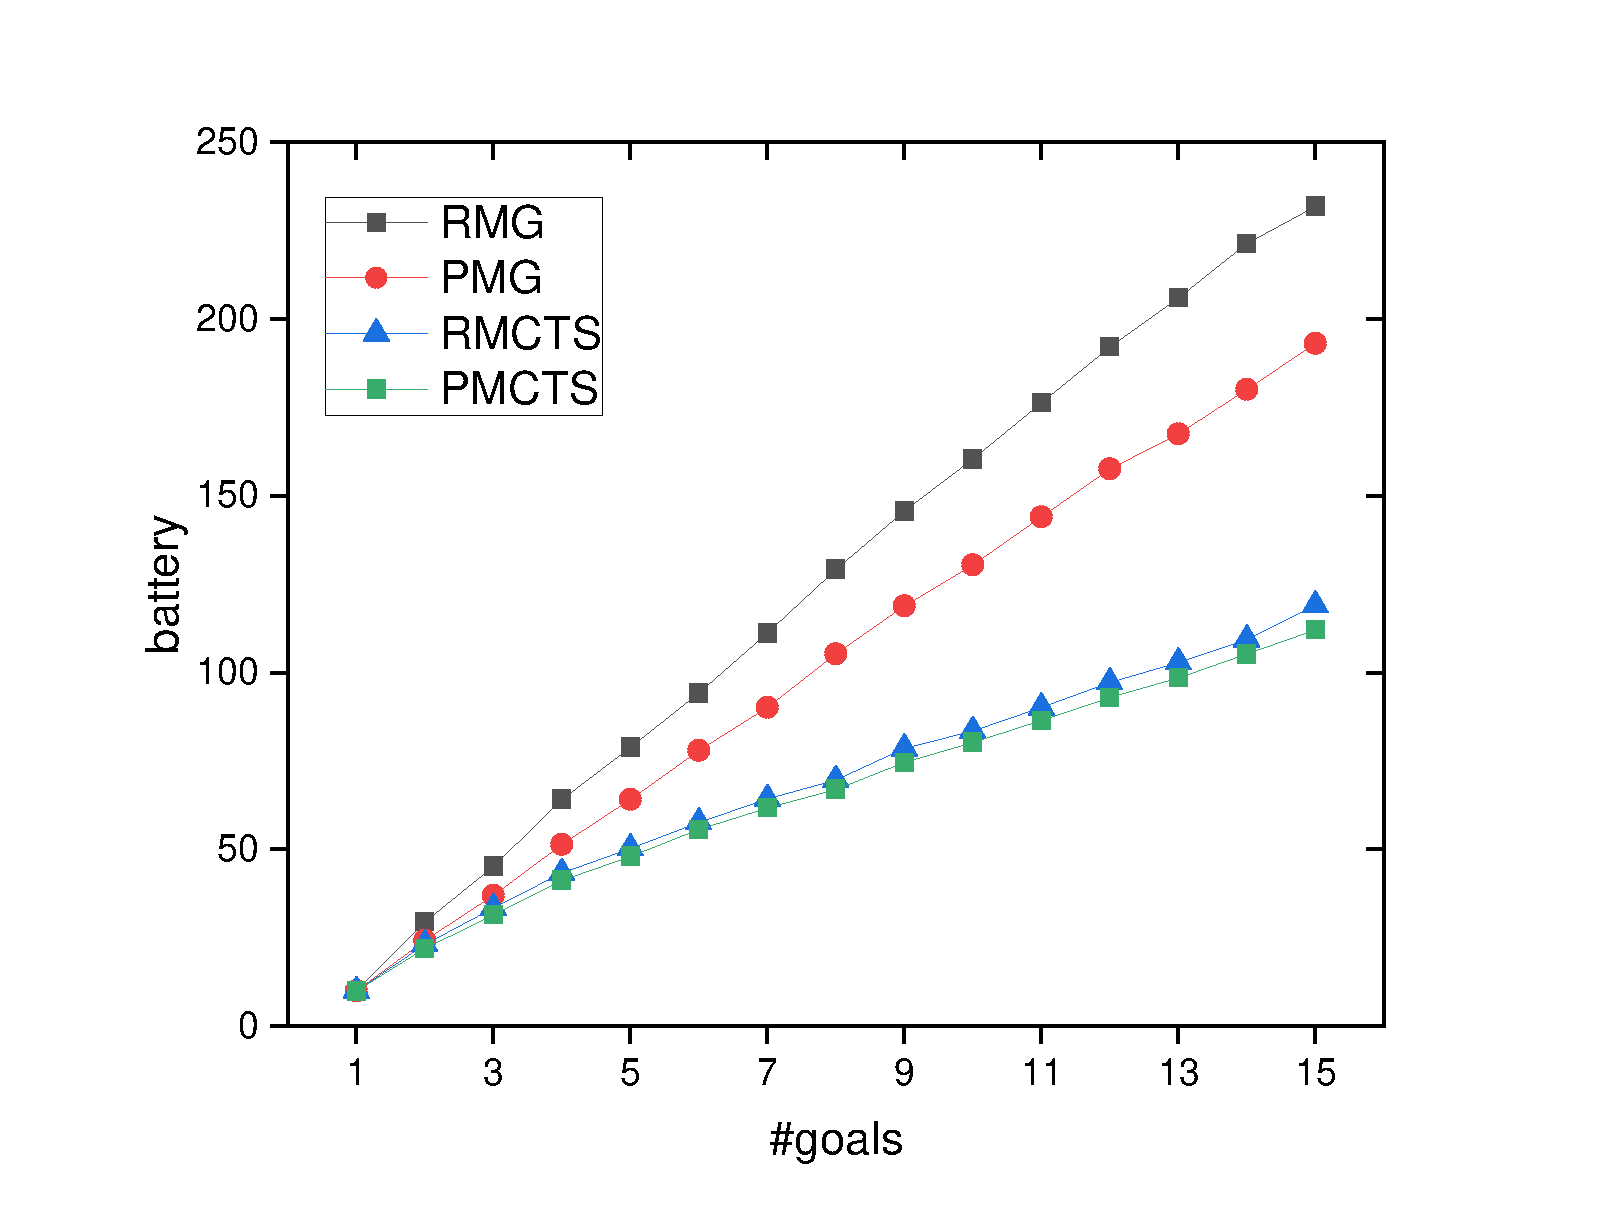
\includegraphics[scale=1]{./figs/gX_cY_fixCap40.pdf}
\captionof{figure}{Battery consumptions with fixed capacity of 40}
\label{fig:static1}
\end{center}\vspace{1cm}

As can be seen, for all approaches the amount of battery consumption increases, as the number of goals increases.
% two baseline
% Natasha: I don't understand the next (commented out) sentence
% general
MCTS-based approaches (PMCTS, and RMCTS) outperform all other approaches, and approaches using proactive maintenance goals have better performance than those using reactive maintenance goals.
%NMCTS has the best performance as it does not consider any battery consumption.
% NMG Natasha: is it NMG or RMG? (comment NMG and text RMG) 
As expected, RMG has the worst performance in all testing cases, i.e., it consumes more battery power than any other approaches.
% reason Natasha: is it NMG or RMG? Change NMG to RMG below
%This is because RMG can only reactively respond to the maintenance goals, causing possible waste of battery when it tries to achieve a goal that is not achievable given the current amount of battery power.
% PMG Natasha: again changed NMG below to RMG
The PMG has better performance than RMG, as it can estimate the battery consumption before pursuing a goal. If the agent will trigger the maintenance goal half way achieving its next achievement goal, then it will choose to recharge first.
% mcts
Finally, both PMCTS and RMCTS have a clear advantage over PMG. Especially, when the given number of goals becomes larger, the differences between MCTS-based approaches and other approaches are more significant. The reason is that the MCTS-based approach can predict not only the possible violation of maintenance conditions during the execution but also possible synergies between different intentions (i.e., the agent can merge the same actions from different intentions to save time and resources).

%----------------------------------------------------------------------------------------
%	CONCLUSIONS
%----------------------------------------------------------------------------------------

\color{SaddleBrown} % SaddleBrown color for the conclusions to make them stand out


\color{DarkSlateGray} % Set the color back to DarkSlateGray for the rest of the content

%----------------------------------------------------------------------------------------
%	FORTHCOMING RESEARCH
%----------------------------------------------------------------------------------------

\section*{Conclusion}
The preliminary results suggested that even without giving any reliable prediction of future violation, \SAM with reactive maintenance goal can still outperform both reactive and proactive approaches proposed in \cite{DuffHT06} in all cases.

The advantage of using \SAM comes from not only the ability to avoid violation between achievement goals and maintenance goals, but also the nature that MCTS can interleave recovery plans and other intentions so as to avoid negative interaction and to exploit synergies 
%as in \cite{Yao/Logan:16a,Yao//:16a} 
if maintenance goals are implemented proactively.

\section*{Future work}
\begin{itemize}
    \item Extend \SAM scheduler to work with nondeterministic actions in uncertain environment.
    \item Extend the current \SAM to additional richer types of goals that are explicitly represented as Linear Temporal Logic formula.
    \item Investigate how to schedule maintenance goals that are only valid for a period of time.
    \item Investigate how to schedule multiple maintenance goals with different priorities or urgency.
\end{itemize}

% One limitation of \SAM is that it doesn't consider uncertainty and estimation errors. Therefore, one potential future work would be to combine the work of \cite{conf/ijcai/0007ALT20} to extend \SAM scheduler to work with nondeterministic actions in uncertain environment.
%
% In future work, it would also be interesting to investigate how to schedule maintenance goals that are only valid for a period of time.
%
% One aspect not addressed in this work is how to schedule multiple maintenance goals with different priorities or urgency. For example, a Mars rover agent may have a maintenance goal to keep its battery level at a certain level and another maintenance goal to avoid collisions. When there is a wall in front of the agent, the goal to avoid collisions will become increasingly urgent.
%
% Yet another potential direction for future work is to extend the current \SAM to additional richer types of goals that are explicitly represented as Linear Temporal Logic formula as proposed in \cite{DastaniRW11}.

%----------------------------------------------------------------------------------------
%	REFERENCES
%----------------------------------------------------------------------------------------

\section*{Acknowledgements}
This work was supported in part by the National Natural Science Foundation of China (61906169) and Yongjiang Talent Introduction Programme (2022A-234-G).

% \nocite{*} % Print all references regardless of whether they were cited in the poster or not
\bibliographystyle{plain} % Plain referencing style
\bibliography{aamas23-mg} % Use the example bibliography file sample.bib

%----------------------------------------------------------------------------------------
%	ACKNOWLEDGEMENTS
%----------------------------------------------------------------------------------------


%----------------------------------------------------------------------------------------

\end{multicols}
\end{document}